\documentclass[11pt,a4paper]{article}
\usepackage[latin1]{inputenc}
\usepackage[spanish]{babel}
\usepackage{amsmath}
\usepackage{amsfonts}
\usepackage{amssymb}
\usepackage{graphicx}
\usepackage[left=2cm,right=2cm,top=2cm,bottom=2cm]{geometry}
\author{Samuel Caleb Mart�nez Hern�ndez}
\begin{document}
\begin{center}
 
\includegraphics[scale=1]{EV/logo.png}
 \end{center} \\ \\
\begin{center}
 {\LARGE Cinem�tica de Robots}
 \end{center} \\
\begin{center}
 {\Large Ing. Mecatr�nica 7-A}
 \end{center} \\ \\
\begin{center}
 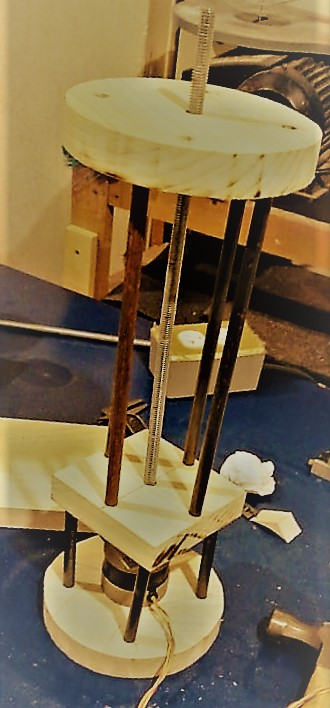
\includegraphics[scale=0.8]{EV/11.jpeg}
 \end{center} \\
\begin{center}
{\Huge REPORTE FINAL S�PTIMO CUATRIMESTRE }
\end{center}\\ \\ \\



\section*{Integrantes del equipo }
* Samuel Caleb Mart�nez Hern�ndez \\
* Fabian Canales Ochoa \\
* Cesar Fabian Flores Macias \\
* Amaury Efrain Gutierrez Chavez \\

\section*{Introducci�n}
De esta manera se concluiremos el ultimo reporte del proyecto robot SCARA, el cual sin duda alguna a resultado ser una grata actividad tanto de aprendizaje como de desarrollo personal acad�mico. \\

\section*{Indice}
	\section{Materias y su utilidad en el proyecto} pagina ... 3\\
	\section{Cronograma de actividades} pagina ... 4\\
	\section{Desarrollo de actividades} pagina ... 4, 5, 6  y  7\\
	\section{Conclusi�n} pagina ... 7\\
	\section{Referencias} pagina ... 7\\

\section*{1.- Materias y su utilidad en el proyecto}
\begin{center}
 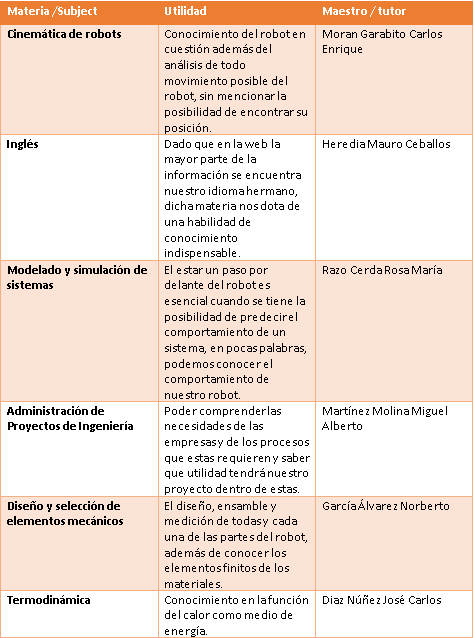
\includegraphics[scale=1]{EV/9.png}
 \end{center} \\
 Como podemos observar, cada materia fue de fundamental ayuda. \\
 
\section*{2.-Cronograma de actividades}
\begin{center}
 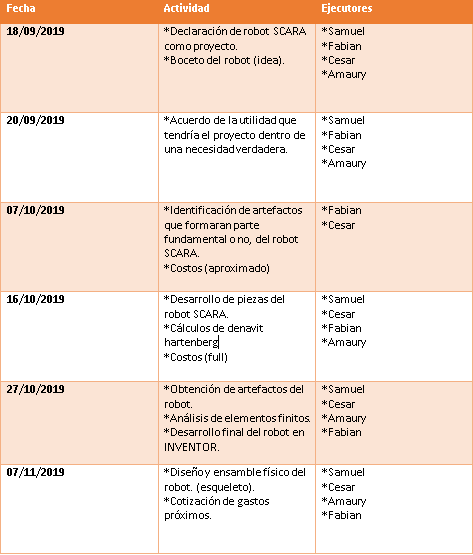
\includegraphics[scale=1]{EV/10.png}
 \end{center} \\
En lo que corresponde a este reporte, se consentrar� en las actividades realizadas desde la fecha del 27 de octubre en adelante. \\

\section*{3.-Desarrollo de actividades }
Cuando se cotizaron los valores monetarios de cada elemento presente en el robot SCARA decidimos que era tiempo de hacernos de los artefactos que serian necesarios inicialmente, para esto, fuimos directamente a un lugar donde sab�amos que sin duda alguna, encontrar�amos lo que necesit�bamos, entre algunas otras cosas. \\

Entre estos artefactos se encuentran... \\

* Tornillos sin fin 35 cm de largo ... 100 pesos mexicanos X 4 \\
* Servo - motores \\ 60 pesos mexicanos c/u \\
* Varillas de acero 3/8 70 pesos mexicanos X 8\\
* Madera de arce 1m X 50 cm \\

Con estos objetos en mano, ya pod�amos trabajar. \\

Antes de empezar a cortar, pegar o cualquier cosa, se realizaron los an�lisis de elementos finitos. A causa de esto, tomamos en cuenta el dise�o del robot, las partes que mas necesitan refuerzos y dimos con una conclusi�n de que podemos hacer para mejorar la resistencia del robot. \\

\begin{center}
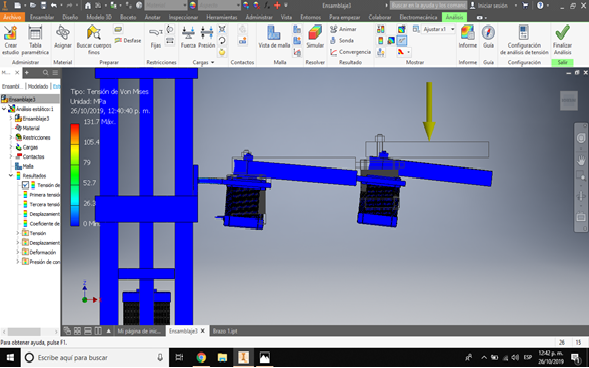
\includegraphics[scale=1]{EV/13.png} 
\end{center}\\

Supimos que a la hora de ensamblar podr�amos encontrar una soluci�n que nos sirva. \\

Comenzamos con una reuni�n del equipo, en el cuela se realizaron diversas tareas. \\
Se realizaron los cortes de la madera para poder de esa forma conseguir las bases de nuestro robot, posteriormente se le hicieron los embones necesarios para colocar las varillas 3/8. utilizamos esta maquina para hacer los cortes iniciales. \\
\begin{center}
 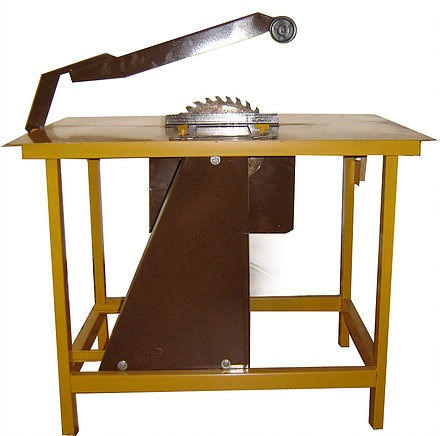
\includegraphics[scale=0.2]{EV/2.jpg}
 \end{center} \\
Una vez se realizaron los cortes principales para separar la pieza beta-alpha, se utilizo la siguiente maquina para poder hacer el circulo con la mejor precisi�n posible. \\
\begin{center}
 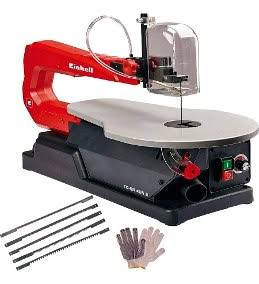
\includegraphics[scale=0.2]{EV/3.jpg}
 \end{center} \\
Por supuesto, no todo en esta vida es perfecto, sin embargo, nosotros esperamos que sea as�, por lo que pasamos la figura a una lija dora mec�nica de mesa, la cual nos sirvi� para que la figura circular nos quedara impecable. \\
\begin{center}
 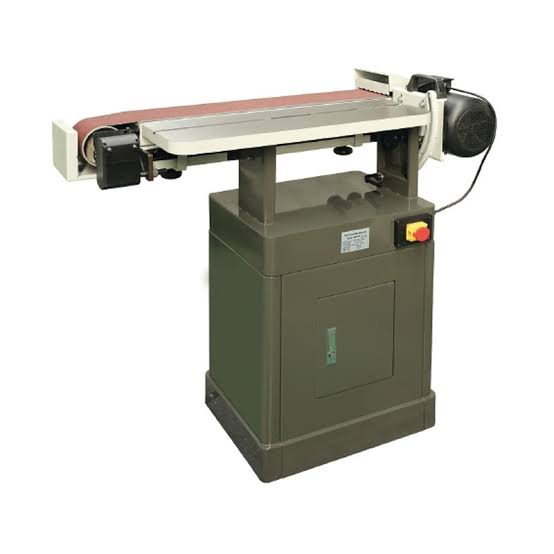
\includegraphics[scale=0.2]{EV/1.jpg}
 \end{center} \\
Posterior a taladrar las piezas para que pueda ser ensamblada, el resultado fue este. \\
\begin{center}
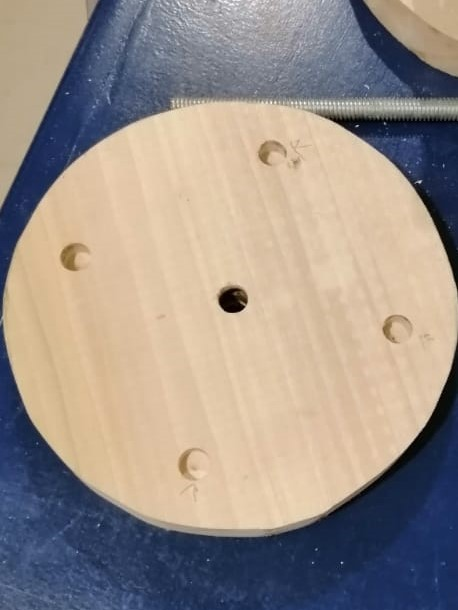
\includegraphics[scale=0.2]{EV/6.jpeg} 
\end{center}\\
El hoyo que se encuentra a medias del circulo de madera nos sirve para poder incrustar el tornillo sin fin...\\
\begin{center}
 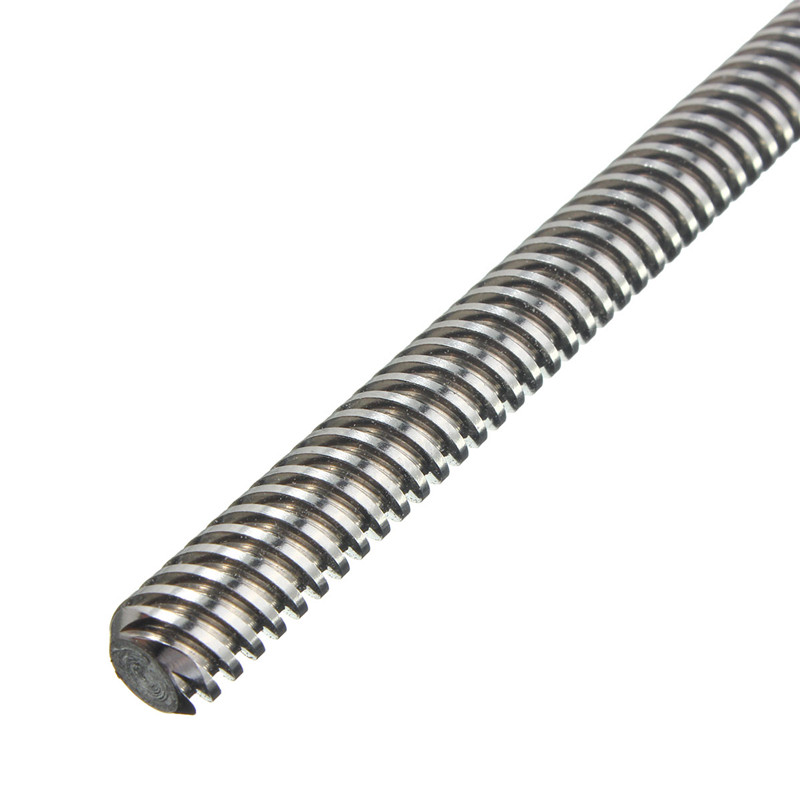
\includegraphics[scale=0.2]{EV/8.jpg}
 \end{center} \\
Qued�ndonos as� el esqueleto del robot SCARA. \\
\begin{center}
 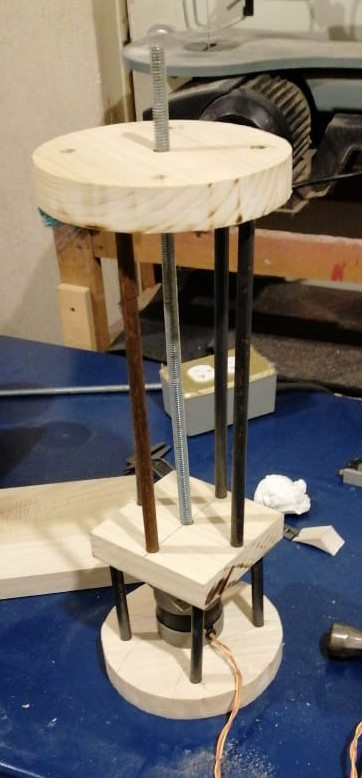
\includegraphics[scale=0.3]{EV/5.jpeg}
 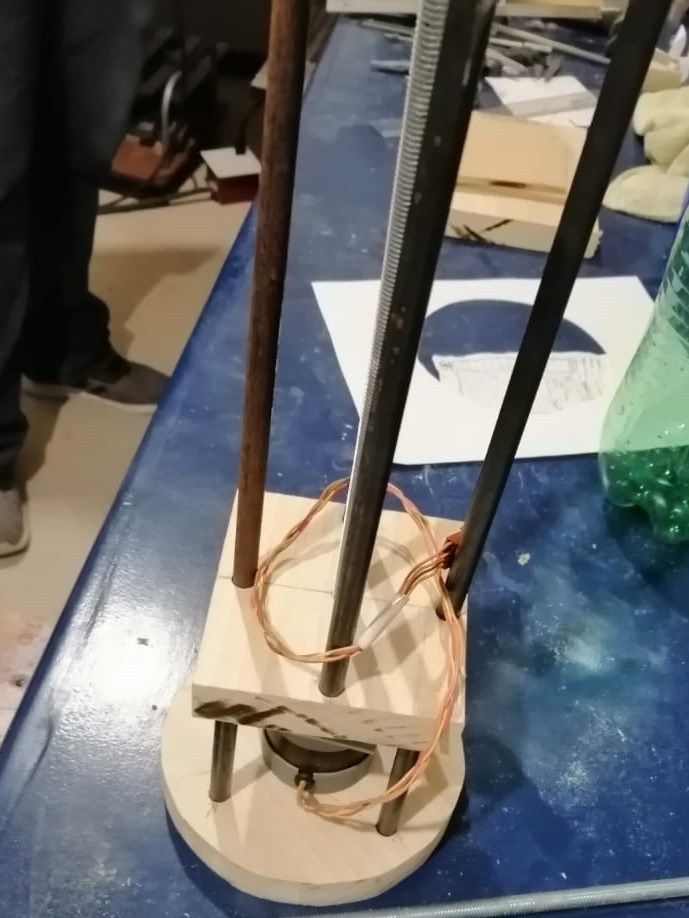
\includegraphics[scale=0.2]{EV/7.jpeg} 
 \end{center} \\
Al final, lo que se espera es que el tornillo sin fin se sold� a la punta del servo motor, dando de esta manera la conclusi�n de la primera  articulaci�n del robot SCARA. Por supuesto que el robot estar�a colocado en la parte inferior del esqueleto, como se puede apreciar en la imagen. \\

Posterior a eso, solo fue cuesti�n de llevarlo con nuestro tutor, osea, nuestro profesor. De esta manera se concluye el ultimo avance realizado al robot SCARA en este cuatrimestre. Por lo menos, los avances en general se suspender�n hasta el siguiente cuatrimestre. \\

\section*{4.- Conclusi�n }
Quiz� no se trate del mejor avance del mundo, sin embargo, contamos con que este inicio nos motive mas adelante, consiguiendo de esta manera ampliar nuestro campo de visi�n en cuanto al numero de posibles a�adidos para el robot. \\

No hay necesidad de preocuparse por lo que ya esta hecho, si no por lo que no se ha hecho aun, ya que este avance resulta muy corto a comparaci�n de lo que nos espera mas adelante, se espera que los conocimientos futuros est�n a la par de las necesidades de nuestro robot, que cabe destacar que, siempre estar� en evoluci�n. \\

\section*{5.- Referencias}
@article{morales2014control,
  title={Control de seguimiento de trayectoria y paletizaci{\'o}n de un robot de tres grados de libertad tipo SCARA (selective compliance assembly robot arm)},
  author={Morales, Luis Alberto and Sotomayor, Nelson Sotomayor and Boada, Yadira},
  journal={Revista Polit{\'e}cnica},
  volume={33},
  number={1},
  year={2014}
}

\end{document}